\documentclass[11pt,a4paper]{article}  % Déclare la classe du document.

\newcommand{\chaptermark}[2]{\og #2 \fg{} (#1)} % ligne uniquement pour éviter une erreur en cas d'article
\include{../1ere-preambule}

\usepackage{epic}   % extension et simplification de  l'environnement picture
\usepackage{graphicx}    % permet d'inclure des graphique externe dans un document
\usepackage{arydshln}   %permet d'avoir des lignes en pointillés

\newcommand{\lignes}[1]{
	\setlength{\unitlength}{1mm}
	\vskip 0,4cm\noindent
	\multido{\i=0+1}{#1}{%
		\noindent
		\begin{picture}(150,5)
			\linethickness{0,005mm}
			\put(-5,0){\dashline{1}(175,5)(5,5)}
		\end{picture}\vskip 0,001cm
	}
	\vskip 0cm
}

\rhead{DS n$^{\circ}02$ - Croissance Linéaire - Suite arithmétique - 13/01/2025}

\newcommand{\va}[1]{\lvert \ #1 \ \rvert}
\newcommand{\vaf}[1]{\left\lvert \ #1\  \right\rvert}

\begin{document}
	\graphicspath{{images/}}
	
	\begin{center}
		
		
		\fbox{
			\begin{minipage}[]{15cm}
				\begin{center}
					\LARGE{\rule{0.5cm}{0pt}\rule[-0.25cm]{0pt}{0.9cm}
						DS n$^{\circ}02$ \\
						Croissance Linéaire - Suite arithmétique 
					}
				\end{center}
			\end{minipage}
		}
	\end{center}

\begin{center}\textbf{1h20min - Barème indicatif}\end{center}
\begin{center}\textbf{Les élèves avec un tier-temps ne traitent pas les questions avec  le symbole \ding{46}}\end{center}
\begin{center}\textbf{Calculatrice autorisée.\\Les résultats devront être justifiés (à l'aide de calcul ou de propriétés).}\end{center}


\exerciceDS{ - (1 points)}
Pour chacune de ces suites arithmétiques définies sur $\mathbb{N}$, calculer $u(10)$.
\begin{multicols}{2}
	\begin{enumMet}
		\item \ding{46} $u(n)=5 n-12$
		\item $u(n)=\dfrac{4 n+7}{3}$
	\end{enumMet}
\end{multicols}

\exerciceDS{ - (3 points)}
Dans chaque cas, $u$ est une suite arithmétique de raison $r$ et de premier terme $u(0)$. Pour les 2 cas, exprimer le terme général de la suite $u(n)$ et calculer le terme de rang 5 .
\begin{multicols}{2}
	\begin{enumMet}
		\item $r=-7$ et $u(0)=3$.
		\item \ding{46} $r=-1,2$ et $u(0)=5,6$.
	\end{enumMet}
\end{multicols}


\exerciceDS{ - (2 points)}
\begin{enumMet}
	\item \ding{46} Voici les premiers termes d'une suite.
	
\begin{tabular}{|Xc|Xc|Xc|Xc|Xc|Xc|}
	\hline$n$ & 1 & 2 & 3 & 4 & 5 \\
	\hline$u(n)$ & 0,25 & 0,58 & 0,91 & 1,24 & 1,57 \\
	\hline
\end{tabular}

Cette suite est-elle une suite arithmétique?

\item Voici les premiers termes d'une suite.

\begin{tabular}{|Xc|Xc|Xc|Xc|Xc|}
	\hline $\boldsymbol{n}$ & 0 & 1 & 2 & 3 \\
	\hline$v(n)$ & 3 & 9 & 27 & 81 \\
	\hline
\end{tabular}

Cette suite est-elle une suite arithmétique?
\end{enumMet}


\exerciceDS{ - (2,5 points)}

$u(n)$ est la suite arithmétique de raison 5 telle que $u(2)=-1$.
\begin{enumMet}
	\item Déterminer $u(0)$;
	\item Exprimer le terme général de la suite $u(n)$.
	\item Calculer le 15ème terme de la suite.
\end{enumMet}

\exerciceDS{ - (2 points)}
$u(n)$ est la suite arithmétique de raison $-2$ telle que $u(3)=10$.
Écrire la liste des termes $u(0)$ à $u(7)$ de cette suite.


\exerciceDS{ - (2,5 points)}

En juin 2022, une rivière de Mayenne a connu une crue exceptionnelle.
Son niveau était $1,5 \mathrm{~m}$ au-dessus de son niveau normal.
Lors de la décrue, le niveau a baissé de 30 cm par jour. On modélise la situation par une suite $u(n)$.
\begin{enumMet}
	\item Montrer que la suite $\left(u(n)\right)$ est arithmétique et préciser sa raison et son premier terme.
	\item Exprimer le terme général de la suite $u(n)$
	\item Si cette évolution se poursuit ainsi, quelle sera la hauteur d'eau au bout de 5 jours
\end{enumMet}

\exerciceDS{ - (3 points)}

Magalie a constaté que chaque année il y a 15 livres de plus dans sa bibliothèque.

Au $1^{\text {er }}$ janvier 2020, elle avait 115 livres.
On note $b_n$ le nombre de livres dans la bibliothèque de Magalie le $1^{\text {er }}$ janvier $2020+n$ où $n \in \mathbb{N}$.
\begin{enumMet}
	\item Montrer que la suite $\left(b_n\right)$ est arithmétique et préciser sa raison et son premier terme.
	\item Exprimer le terme général de la suite $b_n$
	\item Si cette évolution se poursuit ainsi, combien de livres aura Magalie dans sa bibliothèque au $1^{\text {er }}$ janvier 2030 ?
\end{enumMet}

\exerciceDS{ - (4 points)}

Les premiers termes d'une suite $u(n)$ sont représentés dans le graphique ci-dessous:

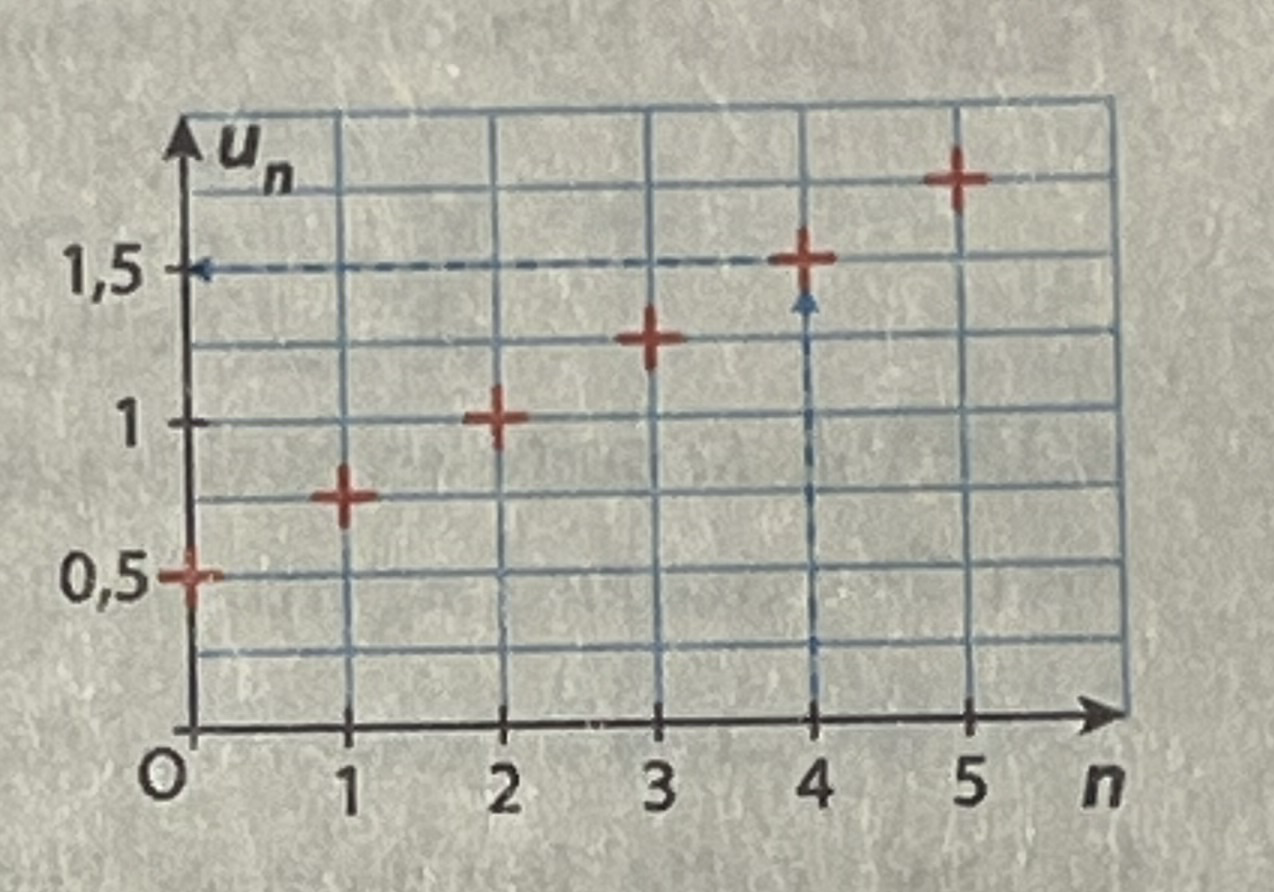
\includegraphics[scale=0.2]{1.OPT.02.03-Img01}

\begin{enumMet}
	\item Donner la valeur du 3ème terme de la suite.
	\item Donner la valeur de $u(5)$.
	\item Montrer que la suite $\left(u(n)\right)$ est arithmétique et préciser sa raison et son premier terme.
	\item En déduire le terme général de la suite.
	\item \ding{46} Donner la valeur du 25ème terme de la suite.
\end{enumMet}



\end{document}

